\newcommand{\standalone}{}
\documentclass[a4paper,11pt,oneside]{book}

%%% το αρχείο αυτό καθορίζει το look που έχουν οι pythonies
%%% γίνεται \input από όλα τα κεφάλαια και τα φύλλα εργασίας

% χρησιμοποιούμενα πακέτα: 
% 
% polyglossia
% xstring
% graphicx
% caption
% xcolor
% hyperref
% minted
% geometry
% titlesec
% datetime
% changepage
% ntheorem

% οριζόμενες εντολές:
%
% smallcaps (βοηθ. removeaccents)
%    μικρά κεφαλαία χωρίς τόνους στα φωνήεντα
% scaling
%    η κλιμάκωση *όλων* των illustrations, τρέχουσα τιμή 0.9
% iconcomputer, iconkeyboard, icondiscuss, iconfillin, iconcaution, iconprompt, dottedline
%    εικονίδια για τα φύλλα εργασίας και εστιγμένη γραμμή
% marginnote
%    πλευρικό σχόλιο
% chapterwabstract (βοηθ. abstract, boxcolor, chaptercolor, concepts, tmpconcepts)
%    εισαγωγικό κείμενο κεφαλαίου με χρωματιστό τετράγωνο, συνοδευτικές έννοιες, κλπ.
% tobecontinued
%    εμφανίζει το "συνεχίζεται στην επόμενη σελίδα"

% οριζόμενα περιβάλλοντα:
% 
% note
%    μια υποσημείωση ή υπόδειξη, με μικρότερα γράμματα
% question
%    μια ερώτηση που "οδηγεί" κάθε νέα ενότητα
% answer
%    μια απάντηση σε μια ερώτηση του φύλλου εργασίας
% theory
%    μια ενότητα "θεωρίας" (στο τέλος ενός κεφαλαίου)
% exercise
%    μια αριθμημένη άσκηση
% step
%    ένα αριθμημένο βήμα (για φύλλο εργασίας)

% για μορφοποίηση κώδικα:
%
% pycode (περιβάλλον)
%     κώδικας python χωρίς αρίθμηση
% pyfile (εντολή)
%     εισαγωγή κώδικα python από αρχείο
% pyfilenl (εντολή)
%     εισαγωγή κώδικα python από αρχείο χωρίς αρίθμηση γραμμών
% pyfilesrc (εντολή)
%    εισαγωγή κώδικα από αρχείο με link στο αρχείο
% pyinline (εντολή)
%     κώδικας python μέσα στη ροή του κειμένου
% pyplain (περιβάλλον, για τα φύλλα εργασίας)
%     κώδικας python χωρίς φόντο
% pynew (περιβάλλον, για τα φύλλα εργασίας)
%     κώδικας python με φόντο
% pyterm (περιβάλλον για τα φύλλα εργασίας)
%     η είσοδος του χρήστη ή τα περιεχόμενα της οθόνης
% pyhighlight (εντολή)
%    highlight κειμένου (χρησιμοποιείται για κώδικα μέσα σε pyplain)


%%% επιλογές γλώσσας και γραμματοσειρών για το XeLaTeX

\usepackage{polyglossia}
\setdefaultlanguage{greek}
\setmainfont[Ligatures=TeX,SmallCapsFont={Linux Libertine O C},SmallCapsFeatures={Letters=SmallCaps}]{Linux Libertine O}
\setsansfont{Linux Biolinum O}
\setmonofont{Ubuntu Mono}
\enablehyphenation

% αφαίρεση τόνων από τα smallcaps
\usepackage{xstring}
\newcommand{\removeaccents}[1]{%
\def\result{#1}%
\StrSubstitute{\result}{ά}{α}[\result]%
\StrSubstitute{\result}{έ}{ε}[\result]%
\StrSubstitute{\result}{ή}{η}[\result]%
\StrSubstitute{\result}{ί}{ι}[\result]%
\StrSubstitute{\result}{ό}{ο}[\result]%
\StrSubstitute{\result}{ύ}{υ}[\result]%
\StrSubstitute{\result}{ώ}{ω}[\result]%
\StrSubstitute{\result}{Ά}{Α}[\result]%
\StrSubstitute{\result}{Έ}{Ε}[\result]%
\StrSubstitute{\result}{Ή}{Η}[\result]%
\StrSubstitute{\result}{Ί}{Ι}[\result]%
\StrSubstitute{\result}{Ό}{Ο}[\result]%
\StrSubstitute{\result}{Ύ}{Υ}[\result]%
\StrSubstitute{\result}{Ώ}{Ω}[\result]%
\result
}

\newcommand{\smallcaps}[1]{\textsc{\removeaccents{#1}}}

%%% εικόνες και λεζάντες

\usepackage{graphicx}
\newcommand{\scaling}{0.9}
\usepackage{caption}
\captionsetup{font=footnotesize}

%%% ειδικά περιβάλλοντα

\usepackage{xcolor}

% ερωτήσεις (που οδηγούν στην επόμενη ενότητα)
\definecolor{questioncolor}{rgb}{0.6,0.5,0.5}
\newenvironment{question}{\noindent\itshape\color{questioncolor}}{\noindent\ignorespaces}

% απαντήσεις (για τις ερωτήσεις των φύλλων εργασίας)
\definecolor{answercolor}{rgb}{0.5,0.5,0.5}
\newenvironment{answer}{\marginnote[16pt]{\iconfillin}\noindent\itshape\color{answercolor}}{\noindent\ignorespaces}

% περιβάλλον "θεωρίας" (πλήρες πλάτος κειμένου)
\usepackage{changepage}
\newenvironment{theory}[1]{\begin{adjustwidth}{}{-\overhang}\smallcaps{#1}\itshape}{\end{adjustwidth}}

% απομεινάρια...
% \newlength{\theoryrulelength}
% \setlength{\theoryrulelength}{36pt}
% \newenvironment{theory}{\rule{\theoryrulelength}{0.4pt}\begin{adjustwidth}{}{-\overhang}\itshape}{\end{adjustwidth}\rule{\theoryrulelength}{0.4pt}}

%%% υπερσύνδεσμοι

\definecolor{linkcolor}{rgb}{0.0,0.5,0.25}
\usepackage[colorlinks=true,urlcolor=linkcolor]{hyperref}

%%% εικονίδια και εστιγμένες γραμμές (για τα φύλλα εργασίας)

\newcommand{\iconcomputer}{
\includegraphics[scale=0.35]{../../share/circle-icons/one-color/computer.eps}}
\newcommand{\iconkeyboard}{
\includegraphics[scale=0.35]{../../share/circle-icons/one-color/keyboard.eps}}
\newcommand{\icondiscuss}{
\includegraphics[scale=0.35]{../../share/circle-icons/one-color/chat.eps}}
\newcommand{\iconfillin}{
\includegraphics[scale=0.35]{../../share/circle-icons/one-color/compose.eps}}
\newcommand{\iconcaution}{
\includegraphics[scale=0.35]{../../share/circle-icons/one-color/caution.eps}}
\newcommand{\iconprompt}{
\includegraphics[scale=0.35]{../../share/circle-icons/one-color/prompt.eps}}
\newcommand{\dottedline}{\vspace{\parskip}\dotfill}

%%% συνεχίζεται στην επόμενη σελίδα

\newcommand{\tobecontinued}{\mbox{}\hfill{\footnotesize ...συνεχίζεται στην επόμενη σελίδα.}}
\newenvironment{note}{\small\upshape}{}

%%% μορφοποίηση κώδικα με το pygmentize

\usepackage{minted}

% fix για ένα bug στο minted που εμφανίζεται όταν χρησιμοποιείται χρώμα στο φόντο (bgcolor)
% http://tex.stackexchange.com/questions/228058/how-to-space-before-and-after-a-minted-code-block-with-bgcolor
\makeatletter
\patchcmd{\minted@colorbg}{\noindent}{\noindent}{}{}
\apptocmd{\endminted@colorbg}{}{}{}
\makeatother

% χρώματα φόντου για τον κώδικα
\definecolor{codebg}{rgb}{0.80,0.95,0.85}
\definecolor{newcodebg}{rgb}{0.75,0.95,0.85}

% ορισμοί για τα περιβάλλοντα κώδικα
% pycode: περιβάλλον κώδικα python χωρίς αρίθμηση
\newminted[pycode]{python3}{bgcolor=codebg}
% pyfile: python από αρχείο
\newmintedfile[pyfile]{python3}{linenos=true,numberblanklines=false,escapeinside=||,bgcolor=codebg}
% pyfilenl: python από αρχείο χωρίς αρίθμηση γραμμών
\newmintedfile[pyfilenl]{python3}{linenos=false,numberblanklines=false,escapeinside=||,bgcolor=codebg}
% pyinline: python μέσα στη ροή του κειμένου
\newmintinline[pyinline]{python3}{linenos=true,numberblanklines=false}
% pyplain: (για τα φύλλα εργασίας) περιβάλλον χωρίς φόντο
\newminted[pyplain]{python3}{bgcolor=white,escapeinside=||,formatcom={\upshape}}
% pynew: (για τα φύλλα εργασίας) περιβάλλον με φόντο
\newminted[pynew]{python3}{bgcolor=newcodebg,escapeinside=||,formatcom={\upshape}}
% pyterm: (για τα φύλλα εργασίας) περιβάλλον για τα περιεχόμενα της οθόνης
\newminted[pyterm]{text}{bgcolor=white,escapeinside=||}

%\newminted[pyterm]{text}{escapeinside=||}
% [TODO] fix: το pyterm χωρίς bgcolor εμφανίζει μεγαλύτερα περιθώρια (πάνω και κάτω) και δεν φαίνεται ωραίο. Το bgcolor είναι προσωρινό workaround, έχει κι αυτό margins (για να μην είναι κολλητά ο κώδικας με το περιθώριο) κι έτσι ο κώδικας στ' αριστερά δεν είναι τέλεια στοιχισμένος.

% εντολή για κώδικα από αρχείο με link στο αρχείο
\newcommand{\pyfilesrc}[2][]{%
\pyfile[#1]{#2}\\
\mbox{}\hfill{\scriptsize\href{http://pythonies.mysch.gr/#2}{\url{#2}}}
}

% εντολή για το highlighting του κώδικα (συνήθως σε pyplain περιβάλλον με escapeinside)
\newcommand{\pyhighlight}[1]{\colorbox{newcodebg}{#1}}

%%% αριθμημένα περιβάλλοντα

\usepackage{ntheorem}

% άσκηση
\makeatletter
\theoremheaderfont{\upshape}%\upshape\bfseries\scshape}
\theorembodyfont{\itshape}%\slshape}
\newtheoremstyle{lmargin}%
  {\item[\theorem@headerfont \llap{##2}\hskip\labelsep\hskip-6pt]}%
  {\item[\theorem@headerfont \llap{##2}\hskip\labelsep ##1\ (##3)\theorem@separator]}
\makeatother
\theoremstyle{lmargin}
\newtheorem{exercise}{}[chapter]

% βήμα φύλλου εργασίας
\makeatletter
\theoremheaderfont{\bfseries}%\upshape\bfseries\scshape}
\theorembodyfont{\upshape}%\slshape}
\newtheoremstyle{lmarginup}%
  {\item[\theorem@headerfont \llap{##2}\hskip\labelsep\hskip-6pt]}%
  {\item[\theorem@headerfont \llap{##2}\hskip\labelsep ##1\ (##3)\theorem@separator]}
\newtheoremstyle{slmarginup}%
  {\item[\theorem@headerfont \llap{##1##2.}\hskip\labelsep\hskip-6pt]}%
  {\item[\theorem@headerfont \llap{##2.}\hskip\labelsep ##1\ (##3)\theorem@separator]}
\makeatother

% deprecated: \newcommand{\standalone}{} to define standalone
%\ifdefined\standalone
    \theoremstyle{slmarginup}
    \newtheorem{step}{}
%\else
%    \theoremstyle{lmarginup}
%    \newtheorem{step}{}[chapter]
%\fi

%%% γεωμετρία σελίδας και συναφείς ορισμοί από το tufte-latex
%%% https://tufte-latex.github.io/tufte-latex/

% εσοχή και διάστημα μεταξύ παραγράφων
% δεν επηρρεάζει το tufte-latex
\parindent=0pt
\parskip=6pt

% γεωμετρία σελίδας και ορισμός μηκών
\usepackage[a4paper,left=24.8mm,top=27.4mm,headsep=2\baselineskip,textwidth=107mm,marginparsep=8.2mm,marginparwidth=49.4mm,textheight=66\baselineskip,headheight=\baselineskip]{geometry}

\setlength{\marginparpush}{12pt}
\addtolength{\marginparpush}{\parskip}
\newlength{\fullwidth}
\setlength{\fullwidth}{\textwidth}
\addtolength{\fullwidth}{\marginparsep}
\addtolength{\fullwidth}{\marginparwidth}
\newlength{\overhang}
\setlength{\overhang}{\marginparsep}
\addtolength{\overhang}{\marginparwidth}

% απομεινάρια...
%\setlength\abovedisplayskip{6pt plus 2pt minus 4pt}
%\setlength\belowdisplayskip{6pt plus 2pt minus 4pt}

% italicize description run-in headings (instead of the default bold)
\renewcommand*\descriptionlabel[1]{\hspace\labelsep\normalfont\em #1}

% πλευρική σημείωση
\newcommand\marginnote[2][0pt]{%
  \marginpar{\hbox{}\vspace*{#1}\vspace*{-1\baselineskip}\noindent \footnotesize\textup{#2}}%
  {}%
}

% formatting title sections
\setcounter{secnumdepth}{-1}

\usepackage{titlesec}
\usepackage[nodate]{datetime}
\newlength{\beforesection}
\setlength{\beforesection}{3ex plus 0.5ex minus 0.2ex}
\addtolength{\beforesection}{-\parskip}
\newlength{\aftersection}
\setlength{\aftersection}{1.5ex plus 0.2ex}
\addtolength{\aftersection}{-\parskip}
\titlespacing*{\section}{0pt}{\beforesection}{\aftersection}

% απομεινάρια...
%\titlespacing*{\chapter}{0pt}{50pt}{40pt}
%\titlespacing*{\section}{0pt}{3.5ex plus 1ex minus .2ex}{2.3ex plus .2ex}

%%% για εισαγωγικό κείμενο κεφαλαίου με χρωματιστό τετράγωνο, συνοδευτικές έννοιες, κλπ.

\newcommand{\abstract}{}
\newcommand{\boxcolor}{}
\newcommand{\chaptercolor}{}
\newcommand{\concepts}{}
\newcommand{\tmpconcepts}{}
\newif\ifbonus

% reference: \titleformat{ command }[ shape ]{ format }{ label }{ sep }{ before-code }[ after-code ]
\titleformat{\chapter}[block]
{\Huge\sffamily}
{}
{0pt}
{\ifbonus\marginnote[-6pt]{\fcolorbox{\boxcolor}{\chaptercolor}{\makebox(40,40){\strut\textcolor{\boxcolor}{\Huge\thechapter}}}\\\vspace{\parskip}\\\tiny\today\\ \currenttime}\else\marginnote[-6pt]{\colorbox{\boxcolor}{\makebox(40,40){\strut\textcolor{\chaptercolor}{\Huge\thechapter}}}\\\vspace{\parskip}\\\tiny\today\\ \currenttime}\fi}
[\small\rmfamily\textmd\abstract\vspace{\parskip}\concepts\vspace{\parskip}\\\mbox{}\hrulefill]

\newcommand{\chapterwabstract}[5]{
	\renewcommand{\abstract}{#2}
    \renewcommand{\tmpconcepts}{#3}
	\ifdefempty{\tmpconcepts}{\renewcommand{\concepts}{}}{\renewcommand{\concepts}{\\\textbf{Έννοιες: }\tmpconcepts}}
	\renewcommand{\boxcolor}{#4}
	\renewcommand{\chaptercolor}{#5}
	\chapter{#1}
}

\definecolor{introColor}{rgb}{0.25,0.5,0.75}
\definecolor{answerColor}{rgb}{0.25,0.75,0.5}
\definecolor{crapsColor}{rgb}{0.5,0.75,0.25}
\definecolor{subtractionColor}{rgb}{0.5,0.25,0.75}
\definecolor{guessColor}{rgb}{0.75,0.25,0.5}
\definecolor{nimColor}{rgb}{0.75,0.5,0.25}
\definecolor{planetColor}{rgb}{0.25,0.25,0.75}
\definecolor{hangmanColor}{rgb}{0.25,0.75,0.25}
\definecolor{oxoColor}{rgb}{0.75,0.25,0.25}

\setcounter{part}{1}
\setcounter{chapter}{2}

\usepackage{booktabs}

%%% DOCUMENT START

\begin{document}

\worksheettrue
\solutionstrue
\chapterwabstract{Mπαρμπούτι}{}{}{crapsColor}{white}

\section{Τυχαιότητα}

Στο παιχνίδι που θα υλοποιήσουμε, ο παίκτης ρίχνει δύο ζάρια. Το αποτέλεσμα του παιχνιδιού εξαρτάται από το \emph{άθροισμα} των ενδείξεων των δύο ζαριών: για κάποιες τιμές του αθροίσματος ο παίκτης κερδίζει, για κάποιες άλλες χάνει, ενώ υπάρχουν και περιπτώσεις που το αποτέλεσμα δεν κρίνεται από την πρώτη ζαριά.

Στην πραγματικότητα, κάθε φορά που ρίχνουμε ένα ζάρι παράγουμε έναν \emph{τυχαίο} αριθμό από το \pyinline{1} μέχρι και το \pyinline{6}. Οι βασικές εντολές της Python δεν μας παρέχουν κάποιο μηχανισμό για να μιμηθούμε αυτή τη διαδικασία.
\marginnote[17pt]{Οι βιβλιοθήκες είναι συλλογές από έτοιμα μικρά προγράμματα που μπορούμε να χρησιμοποιήσουμε στα προγράμματά μας.}
Για το σκοπό αυτό θα χρειαστεί να εισάγουμε στο πρόγραμμά μας μια από τις πολλές διαθέσιμες \emph{βιβλιοθήκες}, τη \pyinline{random}, η οποία παρέχει τη λειτουργικότητα που μας χρειάζεται.

\begin{step}
\emph{Ξεκινήστε} το πρόγραμμα σας με την εντολή που ακολουθεί, για να \emph{εισάγετε} τη βιβλιοθήκη \pyinline{random}:

\begin{pynew}
import random
\end{pynew}

\emph{Προσθέστε} τώρα την εντολή:

\begin{pynew}
dice1 = random.randint(1,6)
\end{pynew}

Στην εντολή αυτή χρησιμοποιείται η \emph{συνάρτηση} \pyinline{randint}, από τη βιβλιοθήκη \pyinline{random}.
Όταν εκτελεστεί το πρόγραμμα, θα παραχθεί μια τυχαία τιμή από το \pyinline{1} μέχρι και το \pyinline{6} και αυτή θα είναι η τιμή της μεταβλητής \pyinline{dice1}.
\end{step}

\begin{step}
Τώρα \emph{προσθέστε} ακόμα μια εντολή που παράγει με τον ίδιο τρόπο την ένδειξη του δεύτερου ζαριού και την ονομάζει \pyinline{dice2}.

\begin{answer}
Θα χρησιμοποιήσουμε ξανά τη \pyinline{randint()}, όπως προηγουμένως και θα αναθέσουμε το αποτέλεσμα που επιστρέφει στη μεταβλητή \pyinline{dice2}:
	
\begin{pynew}
dice2 = random.randint(1,6)
\end{pynew}
\end{answer}
\end{step}

\begin{step}
Στο παιχνίδι αυτό δεν έχουν σημασία οι επιμέρους ενδείξεις των ζαριών, αλλά το \emph{άθροισμά} τους. \emph{Προσθέστε} μια εντολή που υπολογίζει το άθροισμα των \pyinline{dice1} και \pyinline{dice2} και ονομάζει το αποτέλεσμα \pyinline{roll}.

\begin{answer}
Η εντολή που θα προσθέσουμε στο πρόγραμμα είναι:
	
\begin{pynew}
roll = dice1 + dice2
\end{pynew}
\end{answer}
\end{step}

\begin{step}
\emph{Προσθέστε} μια εντολή που εμφανίζει στον παίκτη τη ζαριά που έφερε, δηλαδή τις τιμές των μεταβλητών \pyinline{dice1}, \pyinline{dice2} και \pyinline{roll}.

Για παράδειγμα:

\marginnote[14pt]{\iconcomputer}
\begin{pyterm}
Έριξες 3 και 6 = 9
\end{pyterm}

\begin{answer}
Η εντολή που θα προσθέσουμε στο πρόγραμμα είναι:
	
\begin{pynew}
print("Έριξες",dice1,"και",dice2,"=",roll)
\end{pynew}
\end{answer}

Εκτελέστε το πρόγραμμα μερικές φορές και σημειώστε τις ζαριές σας, όπως εμφανίζονται στην οθόνη.

\begin{answer}
\begin{tabular}{rp{15pt}cp{15pt}cp{15pt}}
\terminline{Έριξες} & \pcenter{\pyinline{1}} & \terminline{και} & \pcenter{\pyinline{5}} & \terminline{=} & \pcenter{\pyinline{6}} \\\addlinespace[\parskip]
\terminline{Έριξες} & \pcenter{\pyinline{2}} & \terminline{και} & \pcenter{\pyinline{1}} & \terminline{=} & \pcenter{\pyinline{3}} \\\addlinespace[\parskip]
\terminline{Έριξες} & \pcenter{\pyinline{4}} & \terminline{και} & \pcenter{\pyinline{6}} & \terminline{=} & \pcenter{\pyinline{10}} \\\addlinespace[\parskip]
\end{tabular}
\end{answer}

Κάθε φορά που εκτελείτε το πρόγραμμα, η ζαριά σας είναι ίδια ή διαφορετική; Υπάρχει τρόπος να γνωρίζετε εκ των προτέρων τη ζαριά που θα φέρετε;

\begin{answer}
Η ζαριά μπορεί να διαφέρει σε κάθε εκτέλεση του προγράμματος ή μπορεί να είναι η ίδια! Ακριβώς επειδή οι αριθμοί των ζαριών είναι τυχαίοι δεν μπορούμε να γνωρίζουμε εκ των προτέρων το αποτέλεσμα.
\end{answer}
\end{step}

\begin{step}
Είναι το ίδιο \emph{πιθανό} να φέρουμε μια ζαριά με άθροισμα \pyinline{7} και μια ζαριά με άθροισμα \pyinline{2};

\begin{note}
Σκεφτείτε πόσοι πιθανοί συνδυασμοί ζαριών αντιστοιχούν στο ένα άθροισμα και πόσοι στο άλλο.
\end{note}

\begin{answer}
Ο μόνος συνδυασμός ζαριών που αντιστοιχεί στο άθροισμα \pyinline{2} είναι το \pyinline{1} και \pyinline{1}. Αντίθετα, το άθροισμα \pyinline{7} προκύπτει από έξι διαφορετικούς συνδυασμούς ζαριών: \pyinline{1} και \pyinline{6}, \pyinline{2} και \pyinline{5}, \pyinline{3} και \pyinline{4} και τα αντίστροφά τους. Επομένως, η πιθανότητα να φέρουμε ζαριά με άθροισμα \pyinline{2} είναι 2 στις 36 (5.56\%), σαφώς μικρότερη από την πιθανότητα να φέρουμε ζαριά με άθροισμα \pyinline{7}, που είναι 6 στις 36 (16.67\%).
\end{answer}

Αντί να παράγουμε δύο ζαριές και να υπολογίζουμε το άθροισμά τους, θα μπορούσαμε να παράγουμε απευθείας ένα τυχαίο άθροισμα, με την εντολή \pyinline{roll = random.randint(2,12)}. Είναι το ίδιο;

\begin{note}
Με τη \pyinline{random.randint(2,12)} όλα τα πιθανά αθροίσματα είναι \emph{ισοπίθανα}.
\end{note}

\begin{answer}
Όχι, γιατί σε αυτή την περίπτωση κάθε ζαριά θα είχε ακριβώς την ίδια πιθανότητα να εμφανιστεί. Δηλαδή στο προηγούμενο παράδειγμα η πιθανότητα να φέρουμε \pyinline{2} ή \pyinline{7} θα ήταν 1 στις 11.
\end{answer}
\end{step}

\section{Ρίξτα!}

Όπως έχει τώρα το πρόγραμμα, τα ζάρια ρίχνονται αμέσως μόλις ξεκινήσει το παιχνίδι. Είναι όμως καλύτερο ν' αποφασίζει ο παίκτης πότε θα ριχτεί η ζαριά, για να του δώσουμε την αίσθηση ότι παίζει.

\begin{step}
\emph{Προσθέστε}, στο σημείο που θεωρείτε κατάλληλο, μια εντολή που θα εμφανίζει στον παίκτη ένα μήνυμα, μια \emph{προτροπή} να ρίξει τα ζάρια πατώντας το πλήκτρο \terminline{ENTER}.

\marginnote[14pt]{\iconcomputer}
\begin{pyterm}
Ρίξε τα ζάρια πατώντας το ENTER...
\end{pyterm}

\begin{answer}
Η εντολή που θα προσθέσουμε στο πρόγραμμα είναι:
	
\begin{pynew}
print("Ρίξε τα ζάρια πατώντας το ENTER...")
\end{pynew}

Ένα πιθανό σημείο για να προσθέσουμε την παραπάνω εντολή είναι μετά από όλες τις εντολές που υπάρχουν ήδη στο πρόγραμμα.

Ένα άλλο πιθανό σημείο είναι πριν την εμφάνιση της προτροπής στον παίκτη να ρίξει τα ζάρια.
\end{answer}

Αμέσως μετά \emph{προσθέστε}:

\begin{pynew}
input()
\end{pynew}

Εκτελέστε το πρόγραμμα. Για ποιο λόγο χρησιμοποιούμε εδώ την \pyinline{input()}; 

\begin{answer}
Η \pyinline{input()} χρησιμοποιείται εδώ, προκειμένου το πρόγραμμα να ``περιμένει'' το πάτημα του  ENTER από τον παίκτη, ώστε να προχωρήσει.
\end{answer}

Γιατί δεν αποδίδεται η τιμή που επιστρέφει η \pyinline{input()} σε κάποια μεταβλητή, όπως γίνεται συνήθως;

\begin{answer}
Διότι η τιμή που πληκτρολογεί στο σημείο αυτό ο χρήστης δεν έχει κάποιο νόημα, πέραν της ``αναμονής'' του προγράμματος. Επομένως, δεν χρειάζεται να την αποδώσουμε σε κάποια μεταβλητή.
\end{answer}

Έχει σημασία αν οι εντολές που μόλις προσθέσατε τοποθετηθούν \emph{πριν} ή \emph{μετά} από τις εντολές που δίνουν τιμή στις \pyinline{dice1} και \pyinline{dice2}; Αν ναι, ποια είναι η διαφορά; 

\begin{answer}
Δεν υπάρχει διαφορά ως προς τις ζαριές ή τα αποτελέσματα που εμφανίζονται στον παίκτη. Απλά αξίζει να σημειωθεί πως αν η \pyinline{input()} μπει μετά από τις εντολές που δίνουν τιμή στις \pyinline{dice1} και \pyinline{dice2}, τότε ουσιαστικά η ζαριά παράγεται πριν το ζητήσει ο παίκτης, το ENTER απλά την εμφανίζει. 
\end{answer}
\end{step}

\section{Πρώτη Εκδοχή}

Τώρα που οι κύβοι ερρίφθησαν, ας εξετάσουμε αν ο χρήστης κέρδισε ή έχασε. Θα ξεκινήσουμε με μια απλή εκδοχή του παιχνιδιού.

\begin{step}
Χρησιμοποιήστε την \pyinline{if} για να ελέγχει το πρόγραμμά σας αν η ζαριά του χρήστη (δηλαδή η τιμή της μεταβλητής \pyinline{roll}) είναι ίση με \pyinline{7}.
Στην περίπτωση αυτή, θα πρέπει να εμφανίζεται το μήνυμα:

\marginnote[16pt]{\iconcomputer}
\begin{pyterm}
Κέρδισες με την πρώτη!
\end{pyterm}

Σε διαφορετική περίπτωση, θα πρέπει να εμφανίζεται το μήνυμα:

%\marginnote[16pt]{\iconcomputer}
\begin{pyterm}
Έχασες με την πρώτη...
\end{pyterm}

\clearpage
\marginnote[24pt]{\iconcaution}
Χρησιμοποιήστε το \pyinline{==} για να ελέγξετε αν δύο τιμές είναι ίσες, όχι το \pyinline{=} που χρησιμοποιείται για να δώσουμε τιμή σε μια μεταβλητή.

\begin{answer}
Οι εντολές που θα προσθέσουμε στο πρόγραμμα είναι:

\begin{pynew}
if roll == 7:
    print("Κέρδισες με την πρώτη!")
else:
    print("Έχασες με την πρώτη...")
\end{pynew}
\end{answer}

Χρησιμοποιήσατε μια \pyinline{if}--\pyinline{else} για να διαχωρίσετε ανάμεσα στις δύο περιπτώσεις ή δύο διαφορετικές \pyinline{if}; Ποια πιστεύετε ότι είναι η διαφορά;

\begin{answer}
Εφόσον οι περιπτώσεις που εξετάζουμε είναι αλληλοαποκλειόμενες, είναι πιο δόκιμο να χρησιμοποιήσουμε την \pyinline{if} -- \pyinline{else}. Με τον τρόπο αυτό όταν η συνθήκη που εξετάζει η \pyinline{if} δεν ισχύει θα εκτελούνται απευθείας οι εντολές που βρίσκονται ``μέσα'' στην \pyinline{else}. Αν χρησιμοποιήσουμε δύο ξεχωριστές \pyinline{if} η κάθε μια θα εξετάζεται ανεξάρτητα από το αν ισχύει ή όχι η προηγούμενη.
\end{answer}

Αν έχετε χρησιμοποιήσει δύο \pyinline{if}, τότε \emph{τροποποιήστε} το πρόγραμμα ώστε να χρησιμοποιεί μια \pyinline{if}--\pyinline{else}. Αυτή είναι η κατάλληλη δομή όταν έχουμε δύο \emph{αμοιβαία αποκλειόμενες} περιπτώσεις, όπως εδώ. 

Εκτελέστε το πρόγραμμα όσες φορές χρειαστεί, μέχρι να φέρετε \pyinline{7}. Η πιθανότητα να γίνει αυτό είναι μία στις έξι, οπότε συνήθως θα χάνετε. Ανακοινώνεται σωστά το αποτέλεσμα σε κάθε περίπτωση;

\begin{note}
Για να ελέγξετε αν το πρόγραμμα λειτουργεί σωστά θα μπορούσατε επίσης να «στήσετε» τη ζαριά, δηλαδή να \emph{παρεμβάλλετε} προσωρινά πριν την \pyinline{if} μια εντολή που δίνει μια διαγνωστική τιμή στην μεταβλητή \pyinline{roll}.
\end{note}

\begin{answer}
Ναι, εμφανίζεται μήνυμα επιτυχίας όταν η ζαριά είναι \pyinline{7} και μήνυμα αποτυχίας σε κάθε άλλη περίπτωση.
\end{answer}
\end{step}

\begin{step}
\emph{Συμπληρώστε} τη συνθήκη της \pyinline{if} έτσι ώστε ο χρήστης να κερδίζει αν φέρει \pyinline{7} \emph{ή} αν φέρει \pyinline{11}.

\marginnote[16pt]{\iconcaution}
Προσέξτε, ο έλεγχος αυτός απαιτεί μια \emph{επιπλέον} συνθήκη σε \emph{διάζευξη} με την υπάρχουσα. Για τη διάζευξη χρησιμοποιήστε τον τελεστή \pyinline{or}.

\begin{answer}
Θα τροποποιήσουμε τη συνθήκη που εξετάζει η \pyinline{if} ως εξής:

\begin{pyplain}
if roll == 7 |\pyhighlight{or roll == 11}|:
    print("Κέρδισες με την πρώτη!")
\end{pyplain}

Ο τελεστής \pyinline{or} συνδέει δύο συνθήκες μεταξύ τους και το αποτέλεσμα είναι αληθές όταν ισχύει οποιαδήποτε από τις δύο (ή και οι δύο).
\end{answer}
\end{step}

\section{Δεύτερη Εκδοχή}

Στην πραγματικότητα, τα πράγματα δεν είναι και τόσο άσχημα για τον παίκτη. Κερδίζει αν φέρει \pyinline{7} ή \pyinline{11}, αλλά χάνει αμέσως μόνο αν φέρει \pyinline{2}, \pyinline{3} ή \pyinline{12}. Σε οποιαδήποτε άλλη περίπτωση, το παιχνίδι, προς το παρόν, θα λήγει ισόπαλο.

Τώρα πια οι διαφορετικές πιθανές εκβάσεις για το παιχνίδι είναι τρεις. Έτσι, για την επέκταση αυτή δεν αρκεί πια η απλή \pyinline{if}--\pyinline{else}, η οποία μπορεί να διακρίνει μόνο ανάμεσα σε δύο περιπτώσεις.

\begin{step}
\emph{Τροποποιήστε} την \pyinline{if} που ελέγχει αν ο παίκτης κέρδισε ή όχι. \emph{Συμπληρώστε} τη συνθήκη που λείπει, έτσι ώστε ο παίκτης να χάνει με την πρώτη αν φέρει \pyinline{2}, \pyinline{3} ή \pyinline{12}:

\begin{pyplain}
if roll == 7 or roll == 11:
    print("Κέρδισες με την πρώτη!")
\end{pyplain}
\begin{pynew}
elif |\textrm{\textit{συνθήκη}}|:   # συμπληρώστε τη συνθήκη
    print("Έχασες με την πρώτη...")
else:
    print("Ισοπαλία.")
\end{pynew}

Η \pyinline{elif} είναι συντομογραφία της \pyinline{else if}. Ελέγχει τη συνθήκη που την συνοδεύει (όπως και η \pyinline{if}) μόνο εφόσον οι συνθήκες που προηγούνται είναι ψευδείς (\pyinline{False}).

\begin{answer}
Η συνθήκη που θα συμπληρώσουμε στην \pyinline{elif} είναι:

\begin{pyplain}
elif |\pyhighlight{roll <= 3 or roll == 12}|:
\end{pyplain}
\end{answer}

Εκτελέστε μερικές φορές το πρόγραμμά σας. Ανακοινώνει σωστά το αποτέλεσμα του παιχνιδιού;

\begin{answer}
Ναι, ανακοινώνει το κατάλληλο μήνυμα ανάλογα με τη ζαριά.
\end{answer}

Η συνθήκη που συμπληρώσατε στην \pyinline{elif} πιστεύετε ότι ελέγχεται κάθε φορά που εκτελείται το πρόγραμμα ή μόνο σε μερικές περιπτώσεις (και πότε);

\begin{answer}
Η συνθήκη της \pyinline{elif} ελέγχεται \emph{μόνο} όταν η συνθήκη που ελέγχει η \pyinline{if} είναι ψευδής (\pyinline{False}).
\end{answer}

\emph{Αντικαταστήστε προσωρινά} την \pyinline{elif} με μια \pyinline{if}. Εκτελέστε μερικές φορές το πρόγραμμα μέχρι να φέρετε \pyinline{7} ή \pyinline{11}.
Τί έχει αλλάξει στην συμπεριφορά του προγράμματος και που πιστεύετε ότι οφείλεται αυτό;

\begin{answer}
Πλέον, ακόμα και στην περίπτωση που ισχύει η συνθήκη της πρώτης \pyinline{if} το πρόγραμμα εξετάζει \emph{και} την περίπτωση της \pyinline{if} που ακολουθεί. Επειδή προφανώς αυτή δεν ισχύει, δηλαδή η ζαριά δεν είναι \pyinline{2},\pyinline{3} ή \pyinline{12}, εκτελούνται οι εντολές της \pyinline{else} και εμφανίζεται \emph{και} το μήνυμα \terminline{Ισοπαλία} μαζί με το μήνυμα \terminline{Κέρδισες με την πρώτη!}
\end{answer}

\marginnote[18pt]{\iconcaution}
Μην ξεχάσετε να \emph{επαναφέρετε} την \pyinline{elif}, ώστε το πρόγραμμα να λειτουργεί και πάλι σωστά.
\end{step}

\section{Τρίτη Εκδοχή}

Ας κάνουμε το παιχνίδι μας πιο ενδιαφέρον και λίγο πιο κοντά στους πραγματικούς κανόνες. Αν ο παίκτης δεν κερδίσει ούτε χάσει με την πρώτη, τότε θα πρέπει να \emph{ξαναρίξει}. Στην περίπτωση αυτή κερδίζει αν η δεύτερη ζαριά του έχει το ίδιο άθροισμα με την πρώτη, ενώ σε διαφορετική περίπτωση χάνει.

\begin{step}
Στο ξεκίνημα της τρίτης περίπτωσης, μετά το \pyinline{else}, \emph{τροποποιήστε} την υπάρχουσα \pyinline{print}, ώστε να ενημερώνει το χρήστη ποια είναι η τιμής της (δεύτερης) ζαριάς που πρέπει να φέρει για να κερδίσει. 

Για παράδειγμα, αν το άθροισμα των ζαριών στην πρώτη προσπάθεια ήταν ίσο με \pyinline{9}, τότε αυτό θα πρέπει να είναι το άθροισμα και στη δεύτερη ζαριά για να κερδίσει ο παίκτης.

\marginnote[16pt]{\iconcomputer}
\begin{pyterm}
Ξαναρίξε. Πρέπει να φέρεις 9
\end{pyterm}

\begin{answer}
Η εντολή \pyinline{print} θα τροποποιηθεί όπως παρακάτω:

\begin{pynew}
print("Ξαναρίξε. Πρέπει να φέρεις", roll)
\end{pynew}
\end{answer}
\end{step}

\begin{step}
%Το πρόγραμμα περιέχει \emph{ήδη} ένα σύνολο εντολών που ``ρίχνουν'' τα δύο ζάρια. 
Το πρόγραμμα περιέχει \emph{ήδη} εντολές που ``ρίχνουν'' τα δύο ζάρια. 

\begin{pyplain}
print("Ρίξε τα ζάρια πατώντας το ENTER...")
input()
dice1 = random.randint(1,6)
dice2 = random.randint(1,6)
roll = dice1 + dice2
print("Έριξες", dice1, "και", dice2, "=", roll)
\end{pyplain}

Στο δικό σας πρόγραμμα είναι πιθανό οι εντολές αυτές να έχουν λίγο διαφορετική σειρά, αλλά αυτό δεν έχει σημασία. Για τη δεύτερη ζαριά χρειαζόμαστε ακριβώς τις ίδιες εντολές.

\emph{Αντιγράψτε} αυτές τις εντολές που αντιστοιχούν στην πρώτη ζαριά του παίκτη και \emph{προσθέστε} τις στο σημείο όπου ο παίκτης πρέπει να ρίξει τη δεύτερη ζαριά του, δηλαδή στην τρίτη περίπτωση όπου ο παίκτης ούτε κερδίζει, ούτε χάνει με την πρώτη.

Εκτελέστε το πρόγραμμα. Σας ζητά να ρίξετε μια δεύτερη ζαριά;

\begin{answer}
Ναι, όταν ο παίκτης δεν κερδίσει ούτε χάσει με την πρώτη, τότε εκτελούνται οι εντολές της \pyinline{else} και το πρόγραμμα ζητά την επανάληψη της ρίψης.
\end{answer}

Εκτελέστε το πρόγραμμα όσες φορές χρειαστεί, μέχρι να τύχει να χάσετε ή να κερδίσετε με την πρώτη ζαριά. Μήπως το πρόγραμμα σας ζητά να ξαναρίξετε, ακόμα και σ' αυτή την περίπτωση;

\begin{answer}
Όχι, δεν συμβαίνει κάτι τέτοιο. Το πρόγραμμα θα εκτελέσει τις εντολές της \pyinline{else} μόνο στην περίπτωση που ο παίκτης δεν κερδίσει ή χάσει με την πρώτη.
\end{answer}

Για ποιο λόγο πιστεύετε ότι μπορεί να εμφανιστεί αυτό το πρόβλημα; Προσπαθήστε ν' απαντήσετε, ακόμα κι αν δεν συνέβη σε σας.

\begin{answer}
Για να παρουσιάσει το πρόγραμμα την παραπάνω ``προβληματική'' συμπεριφορά θα πρέπει οι εντολές που αντιγράψαμε να εκτελούνται σε κάθε περίπτωση, δηλαδή ανεξάρτητα από τη ζαριά του παίκτη. Αυτό θα συμβεί αν δεν προσθέσουμε τις κατάλληλες εσοχές μπροστά από τις εντολές, ώστε να μπουν ``μεσα'' στην \pyinline{else}.
\end{answer}

\marginnote[18pt]{\iconcaution}
Αν το πρόβλημα εμφανίστηκε και στο δικό σας πρόγραμμα, \emph{διορθώστε} το τοποθετώντας τις κατάλληλες \emph{εσοχές} μπροστά από τις εντολές που ξαναρίχνουν το ζάρι, υποδηλώνοντας έτσι ότι αυτές ανήκουν στην τρίτη περίπτωση.
\end{step}

\begin{step}
Τώρα πρέπει να ελεγχθεί αν η δεύτερη ζαριά του παίκτη είναι ίση με την πρώτη, για να διαπιστωθεί αν κέρδισε ή έχασε. 
% Γιατί δεν μπορούμε να κάνουμε αυτόν τον έλεγχο, όπως έχει το πρόγραμμά μας αυτή την στιγμή;
Σε ποια μεταβλητή είναι αποθηκευμένη η τιμή κάθε ζαριάς του παίκτη;
\begin{center}
\begin{tabular}{rp{80pt}p{80pt}}
& \pcenter{πρώτη ζαριά} & \pcenter{δεύτερη ζαριά} \\\addlinespace[2\parskip]
μεταβλητή & \dotfill & \pcenter{\pyinline{roll}}
\end{tabular}
\end{center}

\begin{answer}[]
Στο αποτέλεσμα της πρώτης ζαριάς δίνεται το όνομα \pyinline{roll}.
\marginnote[-8pt]{% 
\center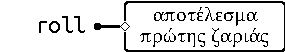
\includegraphics[scale=\scaling]{../illustrations/roll-1.pdf}
\captionof*{figure}{Αρχικά, η τιμή της μεταβλητής \pyinline{roll} αντιστοιχεί στο αποτέλεσμα της πρώτης ζαριάς.}}
Κατά τη δεύτερη ρίψη, χρησιμοποιείται το ίδιο όνομα για το αποτέλεσμα της δεύτερης ζαριάς, με συνέπεια το όνομα \pyinline{roll} ν' αντιστοιχεί πλέον σε αυτή και να μην υπάρχει τρόπος αναφοράς στην πρώτη τιμή.%
\marginnote{% 
\center
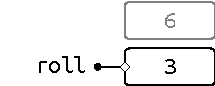
\includegraphics[scale=\scaling]{../illustrations/roll-2.pdf}
\captionof*{figure}{Στη συνέχεια, η \pyinline{roll} χρησιμοποιείται για το αποτέλεσμα της δεύτερης ζαριάς και η τιμή της τροποποιείται. Το αποτέλεσμα της πρώτης ζαριάς δεν είναι πια διαθέσιμο.}}
% Το αποτέλεσμα της πρώτης ζαριάς αποθηκεύεται στη μεταβλητή \pyinline{roll}. Κατά τη δεύτερη ρίψη, χρησιμοποιείται η ίδια μεταβλητή, η \pyinline{roll}, για ν' αποθηκευτεί το αποτέλεσμα της δεύτερης ζαριάς, με συνέπεια η προηγούμενη τιμή να ``επικαλύπτεται'' και να μην είναι πλέον διαθέσιμη.
\end{answer}

Με βάση τον παραπάνω πίνακα, μπορούμε να συγκρίνουμε μεταξύ τους τις δύο τιμές, για να διαπιστώσουμε αν είναι ίσες μεταξύ τους; Αν όχι, πως θα μπορούσαμε να αντιμετωπίσουμε αυτό το πρόβλημα;

\begin{answer}[]
Όχι,%
\marginnote{% 
\center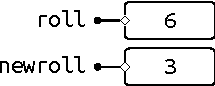
\includegraphics[scale=\scaling]{../illustrations/roll-3.pdf}
\captionof*{figure}{Το αποτέλεσμα της δεύτερης ζαριάς ονομάζεται \pyinline{newroll}. Οι δυο ζαριές, οι τιμές \pyinline{roll} και \pyinline{newroll} μπορούν να συγκριθούν μεταξύ τους.}}
δεν μπορούμε να τις συγκρίνουμε: η τιμή της πρώτης ζαριάς δεν είναι διαθέσιμη. Ούτε έχει νόημα να εξετάσουμε τη συνθήκη \pyinline{roll == roll} μιας και είναι πάντα \pyinline{Αληθής}. Για να διορθώσουμε το πρόβλημα πρέπει να αποθηκεύσουμε το αποτέλεσμα κάθε ζαριάς σε διαφορετική μεταβλητή.
\end{answer}

Στη δεύτερη ζαριά, \emph{τροποποιήστε} τη \pyinline{roll = dice1 + dice2} έτσι ώστε στο νέο άθροισμα των ζαριών να δίνεται διαφορετικό όνομα:

\begin{pyplain}
|\pyhighlight{newroll}| = dice1 + dice2
\end{pyplain}

\emph{Τροποποιήστε} επίσης την \pyinline{print} που ακολουθεί, έτσι ώστε μετά τη δεύτερη ζαριά να εμφανίζεται στο χρήστη το νέο άθροισμα, δηλαδή η τιμή της \pyinline{newroll}.

\begin{answer}
Η εντολή \pyinline{print} θα τροποποιηθεί όπως παρακάτω:

\begin{pynew}
print("Ξαναρίξε. Πρέπει να φέρεις", newroll)
\end{pynew}
\end{answer}

Τώρα η τιμή της κάθε ζαριάς αποθηκεύεται σε διαφορετική μεταβλητή κι έτσι οι δύο τιμές μπορούν να συγκριθούν μεταξύ τους.
\end{step}

\begin{step}
\emph{Προσθέστε} μια \pyinline{if} που θα ελέγχει αν ο παίκτης κέρδισε ή έχασε με τη δεύτερη ζαριά του.
Στην περίπτωση που η δεύτερη ζαριά του παίκτη είναι ίση με την πρώτη, θα πρέπει να εμφανίζεται το μήνυμα:

\marginnote[16pt]{\iconcomputer}
\begin{pyterm}
Έφερες τη ζαριά-στόχο. Κέρδισες!
\end{pyterm}

\clearpage
Σε διαφορετική περίπτωση, θα πρέπει να εμφανίζεται το μήνυμα:

\marginnote[16pt]{\iconcomputer}
\begin{pyterm}
Έφερες διαφορετική ζαριά. Έχασες...
\end{pyterm}

\begin{answer}
Οι εντολές που θα προσθέσουμε στο πρόγραμμα είναι:

\begin{pynew}
if roll == newroll:
    print("Έφερες τη ζαριά-στόχο. Κέρδισες!")
else:
    print("Έφερες διαφορετική ζαριά. Έχασες...")    
\end{pynew}
\end{answer}

Εκτελέστε το πρόγραμμα όσες φορές χρειαστεί, ώστε να κερδίσετε και να χάσετε τουλάχιστον μια φορά \emph{ρίχνοντας και δεύτερη ζαριά}. Ανακοινώνεται σωστά το αποτέλεσμα σε κάθε περίπτωση;

\begin{answer}
Ναι, εμφανίζεται το κατάλληλο μήνυμα σε κάθε περίπτωση.
\end{answer}
\end{step}

\section{Εξαρτήματα}

\begin{step}
\label{step:roll-commands}
Ας \emph{εξετάσουμε} για λίγο ακόμα τις εντολές που σχετίζονται με τη ρίψη των ζαριών:

\begin{pyplain}
print("Ρίξε τα ζάρια πατώντας το ENTER...")
input()
dice1 = random.randint(1,6)
dice2 = random.randint(1,6)
roll = dice1 + dice2
print("Έριξες", dice1, "και", dice2, "=", roll)
\end{pyplain}

Οι εντολές αυτές επαναλαμβάνονται σχεδόν αυτούσιες σε δύο σημεία του προγράμματος. Ουσιαστικά αποτελούν μια \emph{ενότητα εντολών που επιτελούν μια ορισμένη λειτουργία}. 

Ποια μεταβλητή θεωρείτε ότι κρατά το ``αποτέλεσμα'' αυτού του τμήματος κώδικα; Με άλλα λόγια, ποια είναι η τιμή που προκύπτει από αυτόν τον κώδικα και χρησιμοποιείται στο υπόλοιπο πρόγραμμα;

\begin{answer}
Το αποτέλεσμα αποθηκεύεται στη μεταβλητή \pyinline{roll}.
\end{answer}
\end{step}

\begin{step}
Τώρα θα τοποθετήσουμε αυτές τις εντολές μέσα σε μια \emph{συνάρτηση} και στη συνέχεια θα τις ενεργοποιούμε στα σημεία όπου τις χρειαζόμαστε, \emph{καλώντας} την συνάρτηση. Μια συνάρτηση είναι ένα \emph{υποπρόγραμμα} που επιτελεί μια συγκεκριμένη λειτουργία. 

\emph{Προσθέστε} στην αρχή του προγράμματος, κάτω από την \pyinline{import}, τις εντολές που ακολουθούν. Εκτός από την πρώτη και την τελευταία γραμμή, οι υπόλοιπες εντολές υπάρχουν ήδη στο πρόγραμμα, οπότε μπορείτε απλά να τις κάνετε copy--paste:

\clearpage
\marginnote[16pt]{% 
\center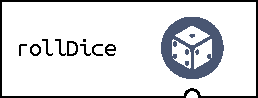
\includegraphics[scale=\scaling]{../illustrations/rollDice.pdf}
\captionof*{figure}{Η συνάρτηση \pyinline{rollDice} είναι ένα ανεξάρτητο τμήμα κώδικα, ένα αυτόνομο ``εξάρτημα'' που επιτελεί μια συγκεκριμένη λειτουργία. Όταν κληθεί, η συνάρτηση προσομοιώνει τη ρίψη δύο ζαριών κι επιστρέφει το άθροισμα των ενδείξεών τους.}}

\begin{pynew}
def rollDice():
    print("Ρίξε τα ζάρια πατώντας το ENTER...")
    input()
    dice1 = random.randint(1,6)
    dice2 = random.randint(1,6)
    roll = dice1 + dice2
    print("Έριξες", dice1, "και", dice2, "=", roll)
    return roll
\end{pynew}

Με τον τρόπο αυτό \emph{ορίζεται} η συνάρτηση \pyinline{rollDice()}, οι εντολές της οποίας υλοποιούν το ``ρίξιμο'' των ζαριών.
Σημειώστε πως το αποτέλεσμα της συνάρτησης, δηλαδή η τιμή της μεταβλητής \pyinline{roll}, \emph{επιστρέφεται} από την συνάρτηση με την εντολή \pyinline{return}.
\end{step}

\begin{step}
Η συνάρτηση \pyinline{rollDice()} είναι σαν ένα μικρό ``εξάρτημα'' που επιτελεί μια συγκεκριμένη λειτουργία. Ωστόσο, αν και την κατασκευάσαμε, δεν την χρησιμοποιούμε πουθενά προς το παρόν.

Στο κύριο πρόγραμμα, στο σημείο όπου ρίχνονται για πρώτη φορά τα ζάρια, \emph{διαγράψτε} τις εντολές του βήματος~\ref{step:roll-commands}, που σχετίζονται με τη ρίψη των ζαριών και \emph{αντικαταστήστε} τις με τη γραμμή:

\begin{pynew}
roll = rollDice()
\end{pynew}

Με τη γραμμή αυτή ενεργοποιούμε ή \emph{καλούμε} την \pyinline{rollDice()}, πραγματοποιώντας έτσι τη ρίψη των ζαριών. Την τιμή που επιστρέφεται από την συνάρτηση, δηλαδή το άθροισμα των ζαριών, την ονομάζουμε \pyinline{roll}.

Εκτελέστε το πρόγραμμα. Λειτουργεί σωστά;

\begin{answer}
Ναι, το πρόγραμμα λειτουργεί σωστά.
\end{answer}

\marginnote[8pt]{\iconcaution}
Σε περίπτωση που κάτι πάει στραβά, βεβαιωθείτε ότι έχετε διαγράψει από το κύριο πρόγραμμα τις εντολές που αντιστοιχούν στο ρίξιμο της πρώτης ζαριάς, αφού αυτές εκτελούνται πλέον όταν καλείται το υποπρόγραμμα. Βεβαιωθείτε επίσης ότι η κλήση του υποπρογράμματος γίνεται στο κατάλληλο σημείο.

Παρατηρεί ο χρήστης κάποια διαφορά στη λειτουργία του προγράμματος, μετά από αυτή την τροποποίηση;

\begin{answer}
Όχι, το πρόγραμμα δεν έχει καμία διαφορά για τον χρήστη, αφού η συνάρτηση κατά την κλήση της εκτελεί ακριβώς τις ίδιες εντολές με προηγουμένως. 
\end{answer}
\end{step}

\begin{step}
\emph{Εντοπίστε} το σημείο του προγράμματος όπου ρίχνονται για δεύτερη φορά τα ζάρια. \emph{Διαγράψτε} τις σχετικές εντολές
%του βήματος~\ref{step:roll-commands}, 
που σχετίζονται με τη ρίψη των ζαριών και \emph{αντικαταστήστε} τις με μια ακόμα κλήση της συνάρτησης \pyinline{rollDice()}. 

\marginnote[18pt]{\iconcaution}
Φροντίστε να αποθηκεύσετε την τιμή που επιστρέφεται από την συνάρτηση στη μεταβλητή \pyinline{newroll}.

\clearpage
\begin{answer}
Η εντολή που θα προσθέσουμε στο πρόγραμμα είναι:

\begin{pynew}
newroll = rollDice()
\end{pynew}
\end{answer}

Εκτελέστε το πρόγραμμα. Λειτουργεί σωστά;

\begin{answer}
Ναι, το πρόγραμμα όσον αφορά τον χρήστη εκτελεί ακριβώς τις ίδιες λειτουργίες με προηγουμένως.
\end{answer}

Τι πιστεύετε ότι κερδίζουμε με την αντικατάσταση των αρχικών εντολών από την κλήση της συνάρτησης \pyinline{rollDice()};

\begin{answer}
Η χρήση των υποπρογραμμάτων έχει το πλεονέκτημα της ``μείωσης'' του κώδικα που γράφει ο προγραμματιστής, αφού χρειάζεται να γράψει τις εντολές μόνο σε ένα σημείο, δηλαδή στο σώμα της συνάρτησης. Στη συνέχεια μπορεί να τις ενεργοποιεί κατά βούληση σε οποιοδήποτε σημείο του προγράμματος, καλώντας απλά τη συνάρτηση. Με τον τρόπο αυτό ο κώδικας γίνεται πιο συμπαγής, ξεκάθαρος και μικρότερος σε έκταση.
\end{answer}
\end{step}

\section{Τελική Εκδοχή}

Στη σημείο αυτό, ο κώδικας του κύριου προγράμματος, μετά τον ορισμό της \pyinline{rollDice()}, πρέπει να μοιάζει κάπως έτσι:

\begin{pyplain}
roll = rollDice()
if roll == 7 or roll == 11:
    print("Κέρδισες με την πρώτη!")
elif roll <= 3 or roll == 12:
    print("Έχασες με την πρώτη...") 
else:
    print("Ξαναρίξε. Πρέπει να φέρεις", roll)
    newroll = rollDice()
    if newroll == roll:
        print("Έφερες τη ζαριά-στόχο. Κέρδισες!")
    else:
        print("Έφερες διαφορετική ζαριά. Έχασες...")
\end{pyplain}

Είμαστε κοντά στην τελική εκδοχή του παιχνιδιού. Στην πραγματικότητα, αν ο παίκτης δεν κερδίσει ούτε χάσει με την πρώτη ζαριά, τότε δεν ξαναρίχνει τα ζάρια μόνο μια φορά αλλά \emph{επαναληπτικά}, μέχρι να φέρει μια ζαριά ίση με την πρώτη του, οπότε κερδίζει. Αν όμως στο μεταξύ, φέρει \pyinline{7}, τότε χάνει.

%%%%%%%%%%%%%%%%%%%%%%%%%%%%%%%%%%%%%%%%%%%%%%%%%%%%%%%%%%%%%%%%%%%

\begin{step}
Στο ξεκίνημα της τρίτης περίπτωσης, όταν δηλαδή το παιχνίδι δεν έχει λήξει από την πρώτη ζαριά, 
\emph{προσθέστε} ``μέσα'' στην \pyinline{else}:

\begin{pynew}
while True:
\end{pynew}

Προσθέστε \emph{τέσσερα κενά} μπροστά από όλες τις εντολές που ακολουθούν τη \pyinline{while}, σηματοδοτώντας έτσι ότι αυτές οι εντολές \emph{εμφωλεύονται} στη \pyinline{while}, δηλαδή περιέχονται σε αυτήν.

\clearpage
\marginnote[16pt]{\iconcaution}
Αν εκτελέσετε το πρόγραμμα και εμφανιστεί μήνυμα σφάλματος του τύπου \terminline{IndentationError: expected an indented block}, τότε ελέγξτε προσεκτικά τις \emph{εσοχές}. H \pyinline{while} πρέπει να βρίσκεται δεξιότερα της \pyinline{else} και οι εντολές που ακολουθούν ακόμα δεξιότερα.

\marginnote[22pt]{Mπορείτε να διακόψετε την εκτέλεση του προγράμματός σας με τον συνδυασμό πλήκτρων \terminline{Ctrl + C}.}
Εκτελέστε το πρόγραμμά σας. Αν κερδίσετε ή χάσετε με την πρώτη ζαριά τότε εκτελέστε το και πάλι. Ποια αλλαγή παρατηρείτε ότι επιφέρει η χρήση της \pyinline{while};

%\marginnote[14pt]{\icondiscuss}
\begin{answer}
Οι εντολές που βρίσκονται μέσα στη \pyinline{while} εκτελούνται επαναληπτικά, δηλαδή ξανά και ξανά. Προς το παρόν η εκτέλεση των εντολών δεν τερματίζεται.
\end{answer}
\end{step}

\begin{step}
\emph{Τροποποιήστε} την \pyinline{if} που βρίσκεται μέσα στην επανάληψη. Η πρώτη περίπτωση δε χρειάζεται αλλαγή: ο παίκτης κερδίζει όταν φέρει την ίδια ζαριά με την αρχική. Ωστόσο, δεν χάνει σε οποιαδήποτε άλλη περίπτωση, αλλά μόνο όταν φέρει \pyinline{7}. 

\begin{pyplain}
        if newroll == roll:
            print("Έφερες τη ζαριά-στόχο. Κέρδισες!")
\end{pyplain}
\begin{pynew}
        elif |\textrm{\textit{συνθήκη}}|:   # συμπληρώστε την συνθήκη
            print("Έφερες 7. Έχασες...")
\end{pynew}

\begin{answer}
Η συνθήκη που θα προσθέσουμε στην \pyinline{elif} είναι:

\begin{pyplain}
elif |\pyhighlight{newroll == 7}|:
\end{pyplain}
\end{answer}

Παρατηρήστε ότι δεν υπάρχει πια η \pyinline{else}. Για ποιο λόγο πιστεύετε ότι συμβαίνει αυτό;

\begin{answer}
Γιατί δεν χρειάζεται πλέον να περιγράψουμε τις ενέργειες που θα εκτελεστούν όταν ο παίκτης δεν φέρει τη ζαριά στόχο ή το \pyinline{7}. Σε αυτή την περίπτωση το πρόγραμμα απλά επαναλαμβάνει τις εντολές που βρίσκονται μέσα στη \pyinline{while}.
\end{answer}

Εκτελέστε το πρόγραμμα. Υπάρχει κάτι που σας ενοχλεί; Κάτι που φαίνεται να μη δουλεύει σωστά;

\begin{answer}
Το πρόγραμμα δεν τερματίζει τη λειτουργία του ακόμα και αν ο παίκτης φέρει τη ζαριά--στόχο ή το \pyinline{7}. Συνεχίζει να τον προτρέπει να ρίξει τα ζάρια.
\end{answer}
\end{step}

\begin{step}
Η εντολή \pyinline{break} διακόπτει την επανάληψη μέσα στην οποία βρίσκεται αμέσως μόλις εκτελεστεί. \emph{Προσθέστε} την \pyinline{break} στο σημείο που θεωρείτε κατάλληλο, έτσι ώστε η επαναληπτική ρίψη των ζαριών να τερματίζεται όταν ο παίκτης ξαναφέρει την αρχική ζαριά--στόχο. 

\begin{answer}
Η εντολή \pyinline{break} θα προστεθεί μέσα στην \pyinline{if} που εξετάζει ότι ο παίκτης έφερε τη ζαριά--στόχο, όπως παρακάτω:

\begin{pyplain}
if newroll == roll:
    print("Έφερες τη ζαριά στόχο. Κέρδισες!")
\end{pyplain}
\begin{pynew}
    break
\end{pynew}
\end{answer}

Εκτελέστε το πρόγραμμα. Αν κερδίσετε ή χάσετε με την πρώτη ζαριά τότε εκτελέστε το και πάλι.
Σταματά η επανάληψη όταν ο παίκτης φέρει τη ζαριά--στόχο σε κάποια από τις επαναλαμβανόμενες ζαριές;

\begin{answer}
Ναι, το πρόγραμμα σταματά.
\end{answer}

\begin{note}
Αν απαντήσατε αρνητικά, τότε βεβαιωθείτε ότι έχετε τοποθετήσει την \pyinline{break} μέσα στην αντίστοιχη περίπτωση της εμφωλευμένης \pyinline{if}.
\end{note}
\end{step}

\begin{step}
\emph{Προσθέστε} την \pyinline{break} στο σημείο που θεωρείτε κατάλληλο, έτσι ώστε η επαναληπτική ρίψη των ζαριών να τερματίζεται όταν ο παίκτης φέρει \pyinline{7}.

\begin{answer}
Η εντολή \pyinline{break} θα προστεθεί μέσα στην \pyinline{elif} που εξετάζει ότι ο παίκτης έφερε \pyinline{7}, όπως παρακάτω:

\begin{pyplain}
elif newroll == 7:
    print("Έφερες 7. Έχασες!")
\end{pyplain}
\begin{pynew}
    break
\end{pynew}
\end{answer}

Εκτελέστε το πρόγραμμα. Σταματά η επανάληψη όταν ο παίκτης φέρει \pyinline{7} σε κάποια από τις επαναλαμβανόμενες ζαριές;

\begin{answer}
Ναι, το πρόγραμμα σταματά όταν ο παίκτης φέρει \pyinline{7}.
\end{answer}
\end{step}
\end{document}
